\documentclass[a4paper,14pt]{extarticle} % the default article class is limited to 12pt, but you can go up to 14, 17 or 20 points if you use the extarticle class
\usepackage{cmap} % make LaTeX PDF output copy-and-pasteable
\usepackage[T2A]{fontenc}
\usepackage[utf8]{inputenc}
\usepackage[english,ukrainian]{babel}

\usepackage{amssymb,amsfonts,mathtools,amsmath,cite,enumerate,float}
\usepackage{indentfirst} % set an additional space before a paragraph at the begining of new section
\usepackage{setspace}
\usepackage{textcomp}

\usepackage{leftidx} % this package enables left subscripts and superscripts in math mode.

\usepackage{import} % for adding a file by path https://tex.stackexchange.com/questions/246/when-should-i-use-input-vs-include

\usepackage{geometry} 
\geometry{left=1.25cm}
\geometry{right=1.25cm}
\geometry{top=1cm}
\geometry{bottom=2cm}

\usepackage[table,xcdraw,dvipsnames]{xcolor}
\usepackage{color}
% 1) tutorial about xcolor:  https://www.overleaf.com/learn/latex/Using_colours_in_LaTeX
% 2) huge tutorial about xcolor: https://latex-tutorial.com/color-latex/ 
% 3) RGB calculator: https://www.w3schools.com/colors/colors_rgb.asp

\usepackage{hyperref}
\definecolor{linkcolor}{HTML}{0000FF}
\definecolor{urlcolor}{HTML}{0000FF} 
\hypersetup{pdfstartview=FitH, unicode=true, linkcolor=linkcolor, urlcolor=urlcolor, colorlinks=true}

\usepackage{graphicx}
\usepackage{wrapfig}
\graphicspath{{Images/}} % path to images

\parskip=1mm % space between paragraphs

\usepackage{listingsutf8} % origin: \usepackage{listings}

\lstset{
    frame=single, %lines
    language=Python,
    aboveskip=3mm,
    belowskip=3mm,
    columns=flexible,
    basicstyle={\small\ttfamily},
    numbers=left,
    numberstyle=\tiny\color{gray},
    commentstyle=\color{OliveGreen},
    stringstyle=\color{Mahogany},
    morestring=[b]''',
    showstringspaces=false,
    keywordstyle=\bfseries\color{blue},
    emph={[1]import, as, for, return}, emphstyle={[1]\bfseries\color{magenta}},
    emph={[2]range}, emphstyle={[2]\bfseries\color{brown}},
    breaklines=true,
    breakatwhitespace=true,
    tabsize=4,
    extendedchars=false, % to use ukrainian text in a code
    inputencoding=utf8 % to use ukrainian text in a code
}

\begin{document}

\import{Title/}{title}

\tableofcontents

\newpage

\subsection*{Завдання та теоретичні основи}
\addcontentsline{toc}{section}{Завдання та теоретичні основи}

Завданням розрахункової роботи є чисельний розв'язок диференціального рівняння в часткових похідних (ДРЧП) одним
з методів: або МСР (методом скінченних різниць), або МСЕ (методом скінчених елементів).

Суть методу сіток (МСР) полягає в апроксимації шуканої неперервної функції сукупністю наближених значень, 
розрахованих в скінченому наборі точок області -- так званих <<вузлах сітки>>. Сукупність вузлів і утворює сітку. 
Використання цього методу дозволяє звести диференціальну граничну задачу або до системи нелінійних рівнянь 
(неявна схема), або до ітераційної формули обчислень відносно невідомих вузлових значень функції (явна схема).

Методи скінчених елементів (МСЕ) і скінчених різниць (МСР) по суті є досить різними. Вони відрізняються за 
сутністю в тому, що в методі скінчених різниць апроксимуються \textit{похідні шуканих функцій}, а в методі
скінчених елементів -- \textit{сам розв’язок}. 

Також методи відрізняються в конструкціях використовуваних сіток: у випадку методу сіток область протікання 
процесу апроксимується прямокутниками, а у випадку методу скінченних елементів -- розбиття з урахуванням 
геометричних особливостей області.

\subsection*{Варіант завдання}
\addcontentsline{toc}{section}{Варіант завдання}

Задається диференціальне рівняння в часткових похідних такого виду:
\begin{equation}
    \frac{\partial u}{\partial t} = a\ \frac{\partial^2 u}{\partial x^2} + b\ \frac{\partial^2 u}{\partial y^2} - cu \label{formula: equation}
\end{equation}

При цьому початкові умови
\begin{align*}
    &\left. u \right|_{t=0}=0 && \text{обрамлення області} \\
    &\left. u \right|_{t=0}=10 && \text{усюди всередині}
\end{align*}

В той час як граничні умови задані таким чином:
\begin{align}
    &\frac{\partial u}{\partial x}=0 && \text{на правій та лівій грані області} \label{formula: mx} \\ \nonumber \\
    &\frac{\partial u}{\partial y}=-ku && \text{на верхній межі} \\ \nonumber \\
    &\frac{\partial u}{\partial y}=ku && \text{на нижній межі} \label{formula: my}
\end{align}

\subsection*{Підготовка моделі до програмної обробки}
\addcontentsline{toc}{section}{Підготовка моделі до програмної обробки}

\subsubsection*{Опис моделі та фізична інтерпретація}
\addcontentsline{toc}{subsection}{Опис моделі та фізична інтерпретація}

Вказане рівняння (\ref{formula: equation}) є рівнянням параболічного типу, яке в загальному випадку виглядає так:
\[ \frac{\partial u}{\partial t} = \sum\limits_i^n k_i\frac{\partial^2 u}{\partial z_i^2} + 
\sum\limits_i^n c_i\frac{\partial u}{\partial z_i} + d_iu +f(z_i,t), \]

де $n$ -- кількість ступенів свободи, а вказані параметри $k_i$, $c_i$, $d_i$, функції $u$ та $f$ мають 
такий зміст:
\begin{align*}
    &u(z_i,t) && \text{стан процесу} \\
    &k_i && \text{коефіцієнт дифузії} \\
    &c_i && \text{коефіцієнт переносу} \\
    &d_i && \text{коефіцієнт <<стоку>>} \\
    &f(z_i,t) && \text{функція джерел}
\end{align*}

ДРЧП виду (\ref{formula: equation}) є типовим прикладом протікання процесу теплопровідності. Крім того, 
оскільки у рівнянні задана залежність від часу та координат, то остаточно робимо висновок про еволюційну 
просторово-розподілену природу заданої моделі розподілу значень стану $u$ (у нашому випадку -- температури) із 
певним значенням в початковий момент часу $t=0$.

\subsubsection*{Дискретизація моделі} 
\addcontentsline{toc}{subsection}{Дискретизація моделі}

Розв'язуватимемо завдання методом скінченних різниць (МСР). Розіб'ємо площину протікання процесу на $n\times n$ 
вузлів. Позначимо індексами $i,j$ номери відповідного рядка та стовпця для конкретно взятого вузла, при цьому 
ці індекси пробігають значення $i=\overline{1,n},\ j=\overline{1,n}$.

Позначимо відстань між сусідніми просторовими вузлами $\Delta x$. Введемо індекс дискретного часу $t$, 
де $t=\overline{1,m}$. І наостанок позначимо відстань між сусідніми моментами часу $\Delta t$.

Скористаймося скінчено-різницевими апроксимаціями для частинних похідних $u_t,u_{xx},u_{yy}$, які, власне, 
є своєрідними модифікаціями їхніх неперервних аналогів:
\begin{align}
    &\frac{\partial u}{\partial t}=\frac{u_{ij}^{t+1} - u_{ij}^{t}}{\Delta x} \label{formula: t} \\ \nonumber \\
    &\frac{\partial^2 u}{\partial x^2}=\lambda\frac{u_{ij+1}^{t+1}-2u_{ij}^{t+1}+u_{ij-1}^{t+1}}{\Delta x^2} 
    + (1-\lambda)\frac{u_{ij+1}^{t}-2u_{ij}^{t}+u_{ij-1}^{t}}{\Delta x^2} \label{formula: x} \\ \nonumber \\
    &\frac{\partial^2 u}{\partial y^2}=\lambda\frac{u_{i+1j}^{t+1}-2u_{ij}^{t+1}+u_{i-1j}^{t+1}}{\Delta y^2} 
    + (1-\lambda)\frac{u_{i+1j}^{t}-2u_{ij}^{t}+u_{i-1j}^{t}}{\Delta y^2} \label{formula: y}
\end{align}

\newpage
Підставимо вирази (\ref{formula: t}), (\ref{formula: x}) та (\ref{formula: y}) у рівняння (\ref{formula: equation}). 
Перенесемо усі компоненти \{t+1\} у ліву частину рівності, а компоненти \{t\} -- у праву. Отримаємо такий 
результат:
\[  u_{ij}^{t+1}(\tfrac{1}{\Delta t}+\tfrac{2a\lambda}{\Delta x^2}+\tfrac{2b\lambda}{\Delta y^2}+c\lambda) - 
    \tfrac{a\lambda}{\Delta x^2}u_{ij+1}^{t+1}-\tfrac{a\lambda}{\Delta x^2}u_{ij-1}^{t+1} - 
    \tfrac{b\lambda}{\Delta y^2}u_{i+1j}^{t+1}-\tfrac{b\lambda}{\Delta y^2}u_{i-1j}^{t+1} = \]
\[  =u_{ij}^t\tfrac{1}{\Delta t} + (1-\lambda)\left(a\ \tfrac{u_{ij+1}^{t}-2u_{ij}^{t}+u_{ij-1}^{t}}{\Delta x^2} + 
    b\ \tfrac{u_{i+1j}^{t}-2u_{ij}^{t}+u_{i-1j}^{t}}{\Delta y^2} - cu_{ij}^t\right) \]

Назагал, чисельним розв'язком диференціального рівняння (\ref{formula: equation}) будуть чергові значення 
функції стану $u$ через певний проміжок часу. Тож у щойно отриманому дискретизованому рівнянні роль невідомих 
змінних відіграють саме компоненти \{t+1\} функції $u$, в той час як значення усіх параметрів та компоненти 
\{t\} функції стану $u$ відомі.

Тож перепозначимо праву частину як одну складену константу $B_{ij}^t$, а компоненти при невідомих змінних 
позначатимемо таким чином: 
\begin{align}
    &a_1 = \tfrac{1}{\Delta t}+\tfrac{2a\lambda}{\Delta x^2}+\tfrac{2b\lambda}{\Delta y^2}+c\lambda \label{formula: a1} \\
    &a_2 = a_3 = -\tfrac{a\lambda}{\Delta x^2} \label{formula: a23} \\
    &a_4 = a_5 = -\tfrac{b\lambda}{\Delta y^2} \label{formula: a45}
\end{align}

Остаточно, з урахуванням виразів (\ref{formula: a1}) - (\ref{formula: a45}) дискретизована модель матиме вид:
\begin{equation} 
    a_1u_{ij}^{t+1} + a_2u_{ij+1}^{t+1} + a_3u_{ij-1}^{t+1} + a_4u_{i+1j}^{t+1} + a_5u_{i-1j}^{t+1} = B_{ij}^t,\quad i,j=\overline{2,n-1} \label{formula: discrete}
\end{equation}

Формула (\ref{formula: discrete}) задає систему лінійних алгебраїчних рівнянь (СЛАР) для кожного наступного 
моменту часу $t$. Проте, варто зауважити, що вираз дає змогу обрахувати виключно внутрішні точки області, в той 
час як самі граничні значення обраховуватимуться дещо інакше.

\subsubsection*{Обробка граничних та початкових умов}
\addcontentsline{toc}{subsection}{Обробка граничних та початкових умов}

Перш за все з'ясуємо, з якої матриці стану варто починати дослідження згідно варіанту. Задання початкових умов 
виразом $\left.u\right|_{t=0}=0$ для граничної області та виразом $\left.u\right|_{t=0}=10$ для усієї внутрішньої 
частини виокремлює матрицю станів в момент часу $t=0$ приблизно такого виду: 
\begin{equation}
u^0=
    \begin{pmatrix}
        0 & 0 & 0 & \ldots & 0 & 0 & 0\\
        0 & 10 & 10 & \ldots & 10 & 10 & 0\\
        0 & 10 & 10 & \ldots & 10 & 10 & 0 \\
        \vdots & \vdots & \vdots & & \vdots & \vdots & \vdots \\
        0 & 10 & 10 & \ldots & 10 & 10 & 0 \\
        0 & 10 & 10 & \ldots & 10 & 10 & 0 \\
        0 & 0 & 0 & \ldots & 0 & 0 & 0 \\
    \end{pmatrix} \label{formula: u0}   
\end{equation}

Наступним кроком дискретизуємо обмеження на границю області.

Аналогічним чином, користуючись скінчено-різницевими апроксимаціями для частинних похідних $u_x$ та $u_y$, 
отримаємо такі дискретизовані аналоги граничних умов (\ref{formula: mx}) - (\ref{formula: my}):
\begin{align*}
    &\frac{u_{i1}^{t+1}-u_{i2}^{t+1}}{\Delta x}=0,\ \frac{u_{in}^{t+1}-u_{in-1}^{t+1}}{\Delta x}=0 && \text{ліві та праві обмеження} \\
    &\frac{u_{1j}^{t+1}-u_{2j}^{t+1}}{\Delta y}=-ku_{1j}^{t+1},\ \frac{u_{nj}^{t+1}-u_{n-1j}^{t+1}}{\Delta y}=ku_{nj}^{t+1} && \text{верхні та нижні обмеження}
\end{align*}

Перенісши невідомі змінні, тобто компоненти \{t+1\}, та коефіцієнти при них у лівий бік, матимемо:
\begin{align}
    &u_{i1}^{t+1}-u_{i2}^{t+1}=0, &&u_{1j}^{t+1}-u_{2j}^{t+1}\left( \tfrac{1}{1+k\Delta y} \right)=0, &i,j = 1 \label{formula: measure1} \\
    &u_{in}^{t+1}-u_{in-1}^{t+1}=0, &&u_{nj}^{t+1}-u_{n-1j}^{t+1}\left( \tfrac{1}{1-k\Delta y} \right)=0, &i,j = n \label{formula: measure2} 
\end{align}

\textbf{Висновок:} дискретизовані записи системи внутрішніх елементів (\ref{formula: discrete}) та граничних елементів 
(\ref{formula: measure1}) - (\ref{formula: measure2}) формуватимуть повну систему лінійних алгебраїчних рівнянь 
(СЛАР). При цьому в програмній реалізації варто враховувати правильний порядок складення цих рівнянь. Озброївшись 
цими формулами, а також початковою матрицею стану (\ref{formula: u0}), покроково розв'язуватимемо СЛАР у пошуках 
чергового значення матриці стану $u$ у кожний наступний момент часу. 

\subsection*{Опис програмної реализації}
\addcontentsline{toc}{section}{Опис програмної реализації}

Порядково зазначу функціонал програми, наведеної на Лістингу \ref{FDM}:
\begin{align*}
    &\texttt{рядки 1-3} && \text{підключення необхідних бібліотек;} \\
    &\texttt{рядки 7-13} && \text{створення початкової матриці стану;} \\
    &\texttt{рядки 5,15,17} && \text{ініціалізація параметрів системи;} \\
    &\texttt{рядки 19-21} && \text{коефіцієнти СЛАР при невідомих змінних;} \\
    &\texttt{рядок 27} && \text{основний ітераційний цикл;} \\
    &\texttt{рядки 39-58} && \text{покроковий обхід граничних умов;} \\
    &\texttt{рядки 60-69} && \text{запис коефіцієнтів СЛАР для внутрішніх елементів;} \\
    &\texttt{рядок 71} && \text{розв'язання сформованої СЛАР;} \\
    &\texttt{рядки 73-83} && \text{перетворення стрічки розв'язку у матричний вигляд;} \\
    &\texttt{рядки 88-109} && \text{візуалізація отриманих результатів.} \\
\end{align*}

Розв'язання СЛАР (рядок 71) виконувалося за допомогою вбудованого методу \texttt{np.linalg.solve()} бібліотеки 
\texttt{numpy}. <<Під капотом>> цей метод використовує для вирішення системи так звану \texttt{LU}-декомпозицію, 
яка в свою чергу є однією з різновидів прямого методу Гауса.

Основна ідея розв'язку системи рівнянь виду $Ax=B$ методом \texttt{LU}-декомпозиції полягає у представленні 
квадратної матриці $A$ у такому вигляді:
\[ A=LU, \]
де $L$ та $U$ -- нижня й верхня трикутна матриця такої ж розмірності. Після такої схеми переупорядкування сам 
розв'язок рівності $Ax=LUx=B$ шукатиметься у два кроки:
\begin{enumerate}
    \item Знаходження розв'язку $y$ з рівняння $Ly=B$;
    \item Знаходження розв'язку $x$ з рівняння $Ux=y$.
\end{enumerate}

Власне, код програми обрахунку ДРЧП, тобто станів системи $u$ у кожен момент часу, наведений нижче:

\lstinputlisting[label = FDM, caption = Код програми]{Code/FDM.py}

\subsection*{Візуалізація отриманих результатів}
\addcontentsline{toc}{section}{Візуалізація отриманих результатів}

Першою буде наведена модель із $15\times 15$ вузлів у різні проміжки часу. Величини параметрів кроків, відповідно 
\[ \Delta x=\Delta y=\Delta t=1, \] значення коефіцієнтів дифузії $ a=2,\ b=1 $, а величина <<стоку>> $ c=-10 $. 
Крім того, заданий параметр для граничних умов $k=0.8$ та величина $\lambda=0.5:$

\begin{figure}[H]
    \begin{minipage}[H]{0.49\linewidth}
        \center{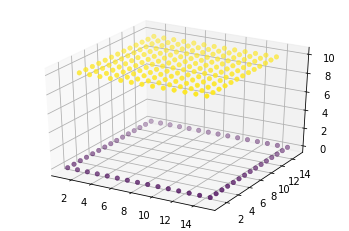
\includegraphics[trim=0in 0in 0.1in 0in, clip, width=1\linewidth]{N15_0.png}} момент $t=0$
    \end{minipage}
    \hfill
    \begin{minipage}[H]{0.49\linewidth}
        \center{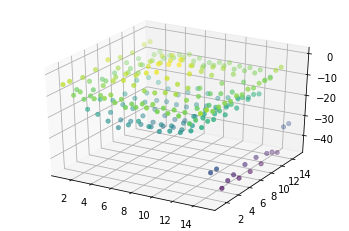
\includegraphics[trim=0in 0in 0.1in 0in, clip, width=1\linewidth]{N15_1.png}} момент $t=1$
    \end{minipage}
\end{figure}

\begin{figure}[H]
    \begin{minipage}[H]{0.49\linewidth}
        \center{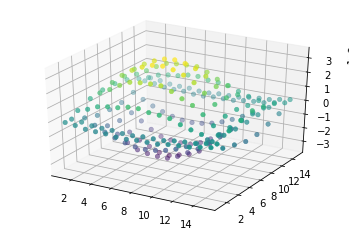
\includegraphics[trim=0in 0in 0.1in 0in, clip, width=1\linewidth]{N15_4.png}} момент $t=4$
    \end{minipage}
    \hfill
    \begin{minipage}[H]{0.49\linewidth}
        \center{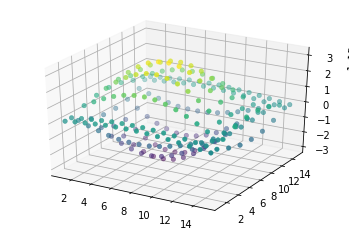
\includegraphics[trim=0in 0in 0.1in 0in, clip, width=1\linewidth]{N15_10.png}} момент $t=10$
    \end{minipage}
    \vfill
    \begin{minipage}[H]{0.49\linewidth}
        \center{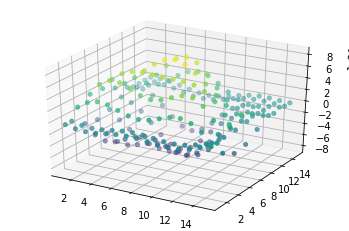
\includegraphics[trim=0in 0in 0.1in 0in, clip, width=1\linewidth]{N15_13.png}} момент $t=13$
    \end{minipage}
    \hfill
    \begin{minipage}[H]{0.49\linewidth}
        \center{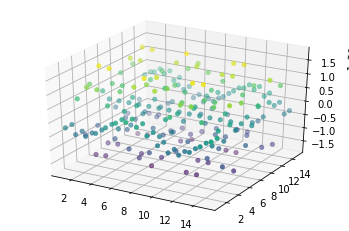
\includegraphics[trim=0in 0in 0.1in 0in, clip, width=1\linewidth]{N15_15.png}} момент $t=15$
    \end{minipage}
\end{figure}

Наступною буде модель із $50\times 50$ вузлів у різні проміжки часу. Аналогічно задані і параметри: величини 
кроків, відповідно \[ \Delta x=\Delta y=\Delta t=1, \] значення коефіцієнтів дифузії $ a=2,\ b=1 $, а 
величина <<стоку>> $ c=-10 $. Крім того, заданий параметр для граничних умов $k=0.8$ та величина $\lambda=0.5:$

\begin{figure}[H]
    \begin{minipage}[H]{0.49\linewidth}
        \center{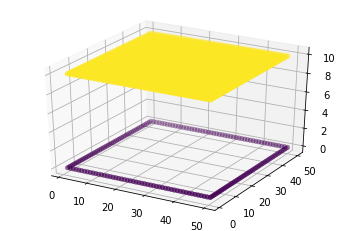
\includegraphics[trim=0in 0in 0.1in 0in, clip, width=1\linewidth]{N50_0.png}} момент $t=0$
    \end{minipage}
    \hfill
    \begin{minipage}[H]{0.49\linewidth}
        \center{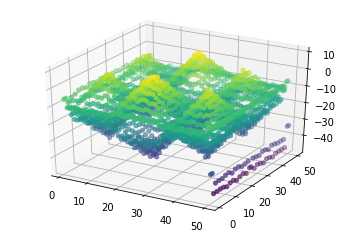
\includegraphics[trim=0in 0in 0.1in 0in, clip, width=1\linewidth]{N50_1.png}} момент $t=1$
    \end{minipage}
\end{figure}

\begin{figure}[H]
    \begin{minipage}[H]{0.49\linewidth}
        \center{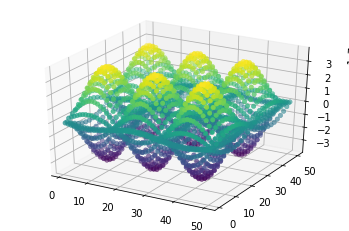
\includegraphics[trim=0in 0in 0.1in 0in, clip, width=1\linewidth]{N50_3.png}} момент $t=3$
    \end{minipage}
    \hfill
    \begin{minipage}[H]{0.49\linewidth}
        \center{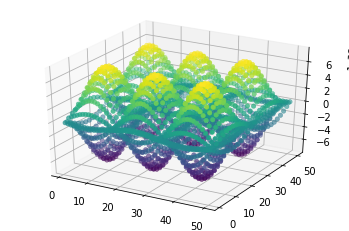
\includegraphics[trim=0in 0in 0.1in 0in, clip, width=1\linewidth]{N50_12.png}} момент $t=12$
    \end{minipage}
\end{figure}

\subsection*{Висновки}
\addcontentsline{toc}{section}{Висновки}

У роботі було розглянуто розв'язання диференціального рівняння у часткових похідних (ДРЧП) методом скінченних 
різниць (МСР), також відомим як метод сіток. Спершу над заданою областю рівняння параболічного типу була проведена 
дискретизація на певну кількість вузлів. Опісля після обробки початкових та граничних умов було остаточно 
створене підґрунтя для формування системи алгебраїчних лінійних рівнянь (СЛАР), розв'язком якої є матриця 
станів у поточний момент часу.

Щодо програмного етапу, розв'зок СЛАР виконувався за допомогою вбудованого методу \texttt{np.linalg.solve()} 
бібліотеки \texttt{numpy}. <<Під капотом>> цей метод використовує так звану \texttt{LU}-декомпозицію, 
яка в свою чергу є однією з різновидів прямого методу Гауса. З обрахункової точки зору, при кількості вузлів 
$15\times 15$ час однієї ітерація сягав $0.25\text{ c}$, в той час як для $50\times 50$ вузлів -- $1.55\text{ c}$.

У результатах роботи наведено приклади візуалізації нестійкої (перша модель) та стійкої (друга модель) схем. 
Проте, при інших значенях параметрів (наприклад, задовільнивши критерій Куранта значеннями $a=1,\ b=0.9$ замість 
$a=2,\ b=1$), можна досягнути стійкого аналогу для першої візуалізації. 

\end{document}